\documentclass{article}
\usepackage{../latex-course}
\usepackage{week-06}

\courseweek{06}{Tables and Floats}
\coursestudents{Name 1 \and Name 2}

\title{The Chambolle--Pock Algorithm for Image Denoising}
\author{Name 1 (Matriculation Nr 1), Name 2 (Matriculation Nr 2)}
\begin{document}
\maketitle

\section{Total-Variation Denoising}
\label{section:problem}
A grayscale image can be represented as a vector $x \in \R^n$ that stores one intensity per pixel, with intensities scaled to $[0, 1]$.
A clean photograph $x^*$ can incorrectly be recorded as $b = x^* + \eta$ with additive noise $\eta$, and denoising is the task of recovering the clean image $x^*$.
\zcref[S]{figure:denoising} shows the three images involved for a classic testpiece.
Simply averaging neighbouring pixels would remove the grainy noise but also wash out the edges.
The Rudin--Osher--Fatemi approach proposes finding a suitable denoised version of an image by optimizing a weighted sum of the distance of the denoised and the noisy image and a penalty term for the \emph{total variation} of the denoised image $x$,
\begin{equation}
	\label{eq:rof}
	\min_{x \in \R^n} \; \tfrac12 \norm{x - b}_2^2 + \lambda \norm{\nabla x}_{2,1},
	\qquad
	\norm{\nabla x}_{2,1} = \sum_i \norm{(\nabla x)_i}_2,
\end{equation}
where $\nabla$ is the discrete image gradient and $\lambda > 0$ trades data fidelity against smoothness.
The total-variation term is convex but \emph{non-smooth}, i.e., the pixel norm $\norm{(\nabla x)_i}_2$ has no derivative where $(\nabla x)_i = 0$, which is exactly on the denoised flat regions the model is meant to produce.
Plain gradient descent, which needs first-order derivatives, therefore cannot be applied.
The Chambolle--Pock algorithm instead treats~\eqref{eq:rof} as a min-max problem and advances each part by a proximal step.

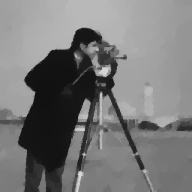
\includegraphics[width = 0.3\linewidth]{cameraman-cp}
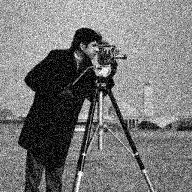
\includegraphics[width = 0.3\linewidth]{cameraman-noisy}
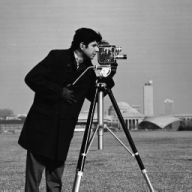
\includegraphics[width = 0.3\linewidth]{cameraman}

\section{Min-Max Reformulation and the Chambolle--Pock Algorithm}
\label{section:algorithm}
The discrete gradient $K = \nabla$ maps $\R^n$ into the space $Y = (\R^2)^n$ of dual vector fields, one $2$-vector per pixel.
Rewriting~\eqref{eq:rof} as $\min_{x \in \R^n} F(K x) + G(x)$ with the regularizer $F(z) = \lambda \norm{z}_{2,1}$ carrying the weight $\lambda > 0$ of~\eqref{eq:rof} and the data term $G(x) = \tfrac12 \norm{x - b}_2^2$, and expressing $F(K x) = \max_{p \in Y} \dual{K x}{p} - F^*(p)$ through the convex conjugate $F^*$, turns the model into the min-max problem
\begin{equation}
	\label{eq:minmax}
	\min_{x \in \R^n} \; \max_{p \in Y} \; \dual{\nabla x}{p} + G(x) - F^*(p),
	\qquad
	\text{where}
	\quad
	F^*(p) = \delta_{\{\, \norm{p}_{2,\infty} \le \lambda \,\}}(p).
\end{equation}
Here $\delta$ is the indicator function, so $F^*$ confines the dual variable $p$ to the ball $\norm{p}_{2,\infty} \le \lambda$ in the norm $\norm{p}_{2,\infty} = \max_i \norm{p_i}_2$.
The induced dual proximal map is the pixelwise projection onto that ball, $[\proj_\lambda(q)]_i = q_i / \max\{1, \norm{q_i}_2 / \lambda\}$.
\zcref[S]{algorithm:cp} alternates a proximal ascent step in $p$ with a proximal descent step in $x$ and over-relaxes the primal variable.
Both proximal maps are explicit, as \zcref{table:ingredients} records.
We use the matched steps $\tau = \sigma = 1/\sqrt{8}$, which satisfy $\tau \sigma L^2 \le 1$ because $L = \norm{\nabla}_2 \le \sqrt{8}$, and the full over-relaxation $\theta = 1$, for which the ergodic iterates close the primal--dual gap at the rate $\mathcal{O}(1/N)$.

\begin{algorithm}[htbp]
	\caption{Chambolle--Pock for the ROF denoising model~\eqref{eq:rof}.}
	\label{algorithm:cp}
	\begin{algorithmic}[1]
		\Require noisy image $b$, weight $\lambda > 0$, steps $\tau, \sigma > 0$ with $\tau \sigma L^2 \le 1$, relaxation $\theta \in [0, 1]$
		\Ensure a denoised image $x$
		\State $x \gets b$, \enspace $\bar{x} \gets b$, \enspace $p \gets 0$
		\While{stopping criterion not satisfied}
			\State $p \gets \proj_\lambda\paren*{p + \sigma \, \nabla \bar{x}}$
				\Comment{dual ascent and clip}
			\State $x^{+} \gets \dfrac{x + \tau \, \dvg p + \tau \, b}{1 + \tau}$
				\Comment{primal descent}
			\State $\bar{x} \gets x^{+} + \theta \paren*{x^{+} - x}$
				\Comment{over-relaxation}
			\State $x \gets x^{+}$
		\EndWhile
		\State \Return $x$
	\end{algorithmic}
\end{algorithm}

	The ingredients of the min-max form~\eqref{eq:minmax} of the ROF model, and the proximal and adjoint maps that \zcref{algorithm:cp} evaluates.
	%{@{} l >{$}l<{$} >{$}l<{$} @{}}
	\begin{alignat}{3}
		Role & \text{Term} & \text{Proximal or adjoint map} \\
		data fidelity G   & G(x) = \tfrac12 \norm{x - b}_2^2        & \prox_{\tau G}(z) = \dfrac{z + \tau b}{1 + \tau} \\
		regularizer F     & F(\nabla x) = \lambda \norm{\nabla x}_{2,1} & \prox_{\sigma F^*}(q) = \proj_\lambda(q) \\
		operator K        & K = \nabla                             & K^* = -\dvg \\
		operator norm L   & L = \norm{\nabla}_2 \le \sqrt{8}        & \tau \sigma L^2 \le 1 \\
	\end{alignat}
\section{A Numerical Experiment}
\label{section:experiment}
We run \zcref{algorithm:cp} on the cameraman image of \zcref{figure:denoising}.
The noisy data in \zcref{figure:noisy} have a peak signal-to-noise ratio (PSNR) of \qty{20.4}{\decibel}; after \num{120} iterations the output in \zcref{figure:output} reaches \qty{26.5}{\decibel}, suppressing the noise while keeping the camera, the tripod and the skyline sharp -- the piecewise-constant look typical of total variation.
\zcref[S]{table:results} shows the results for the experiment repeated at three noise levels~$\nu$, with the weight $\lambda$ tuned to each.
Stronger noise needs a larger~$\lambda$ and leaves a lower final PSNR, and the mild staircasing of total variation then becomes visible in the flat sky.

	Chambolle--Pock denoising of the cameraman image ($192 \times 192$ pixels) at three noise levels: the total-variation weight~$\lambda$, the matched steps $\tau = \sigma = 1/\sqrt{8}$, the number of iterations, the PSNR of the noisy data and of the reconstruction, the final primal energy of~\eqref{eq:rof}, the run time, and a remark on the result.
	\begin{alignat}{7}
		& & & & PSNR (\unit{\decibel}) & & & \\
		{Noise \nu} & {\lambda} & {\tau = \sigma} & {Iters.} & {Noisy} & {Denoised} & {Energy} & {Time \unit{\second}} & {Remark} \\
		0.05 & 0.06 & 0.35 & 120 & 26.24 & 29.92 & 108.4 & 1.72 & light noise, edges intact \\
		0.10 & 0.12 & 0.35 & 120 & 20.39 & 26.48 & 268.6 & 2.00 & the setting of \zcref{figure:denoising} \\
		0.15 & 0.17 & 0.35 & 120 & 17.00 & 24.56 & 482.4 & 2.87 & mild staircasing in flat areas \\
	\end{alignat}
\end{document}
